\documentclass[a4paper, 12pt]{article}

% packages
\usepackage{amssymb}
\usepackage[fleqn]{mathtools}
\usepackage{tikz}
\usepackage{enumerate}
\usepackage{bussproofs}
\usepackage{xcolor}
\usepackage[margin=1.3cm]{geometry}
\usepackage{logicproof}
\usepackage{diagbox}
\usepackage{listings}
\usepackage{graphicx}
\usepackage{lstautogobble}
\usepackage{hyperref}
\usepackage{multirow}
\usepackage{tipa}
\usepackage{pgfplots}

% tikz libraries
\usetikzlibrary{
    decorations.pathreplacing,
    arrows,
    shapes.gates.logic.US,
    circuits.logic.US,
    calc,
    automata,
    positioning,
    intersections
}

\pgfplotsset{compat=1.16}

\pgfmathdeclarefunction{gauss}{2}{%
  \pgfmathparse{1/(#2*sqrt(2*pi))*exp(-((x-#1)^2)/(2*#2^2))}%
}

\allowdisplaybreaks % allow environments to break
\setlength\parindent{0pt} % no indent

% shorthand for verbatim
% this clashes with logicproof, so maybe fix this at some point?
\catcode`~=\active
\def~#1~{\texttt{#1}}

% code listing
\lstdefinestyle{main}{
    numberstyle=\tiny,
    breaklines=true,
    showspaces=false,
    showstringspaces=false,
    tabsize=2,
    numbers=left,
    basicstyle=\ttfamily,
    columns=fixed,
    fontadjust=true,
    basewidth=0.5em,
    autogobble,
    xleftmargin=3.0ex,
    mathescape=true
}
\newcommand{\dollar}{\mbox{\textdollar}} %
\lstset{style=main}

% augmented matrix
\makeatletter
\renewcommand*\env@matrix[1][*\c@MaxMatrixCols c]{%
\hskip -\arraycolsep
\let\@ifnextchar\new@ifnextchar
\array{#1}}
\makeatother

% ceiling / floor
\DeclarePairedDelimiter{\ceil}{\lceil}{\rceil}
\DeclarePairedDelimiter{\floor}{\lfloor}{\rfloor}

% custom commands
\newcommand{\indefint}[2]{\int #1 \, \mathrm{d}#2}
\newcommand{\defint}[4]{\int_{#1}^{#2} #3 \, \mathrm{d}#4}
\newcommand{\pdif}[2]{\frac{\partial #1}{\partial #2}}
\newcommand{\dif}[2]{\frac{\mathrm{d}#1}{\mathrm{d}#2}}
\newcommand{\limit}[2]{\raisebox{0.5ex}{\scalebox{0.8}{$\displaystyle{\lim_{#1 \to #2}}$}}}
\newcommand{\limitsup}[2]{\raisebox{0.5ex}{\scalebox{0.8}{$\displaystyle{\limsup_{#1 \to #2}}$}}}
\newcommand{\summation}[2]{\sum\limits_{#1}^{#2}}
\newcommand{\product}[2]{\prod\limits_{#1}^{#2}}
\newcommand{\intbracket}[3]{\left[#3\right]_{#1}^{#2}}
\newcommand{\laplace}{\mathcal{L}}
\newcommand{\fourier}{\mathcal{F}}
\newcommand{\mat}[1]{\boldsymbol{#1}}
\renewcommand{\vec}[1]{\boldsymbol{#1}}
\newcommand{\rowt}[1]{\begin{bmatrix}
    #1
\end{bmatrix}^\top}
\DeclareMathOperator*{\argmax}{argmax}
\DeclareMathOperator*{\argmin}{argmin}

\newcommand{\lto}[0]{\leadsto\ }

\newcommand{\ulsmash}[1]{\underline{\smash{#1}}}

\newcommand{\powerset}[0]{\wp}
\renewcommand{\emptyset}[0]{\varnothing}

\makeatletter
\newsavebox{\@brx}
\newcommand{\llangle}[1][]{\savebox{\@brx}{\(\m@th{#1\langle}\)}%
  \mathopen{\copy\@brx\kern-0.5\wd\@brx\usebox{\@brx}}}
\newcommand{\rrangle}[1][]{\savebox{\@brx}{\(\m@th{#1\rangle}\)}%
  \mathclose{\copy\@brx\kern-0.5\wd\@brx\usebox{\@brx}}}
\makeatother
\newcommand{\lla}{\llangle}
\newcommand{\rra}{\rrangle}
\newcommand{\la}{\langle}
\newcommand{\ra}{\rangle}
\newcommand{\crnr}[1]{\text{\textopencorner} #1 \text{\textcorner}}
\newcommand{\bnfsep}[0]{\ |\ }
\newcommand{\concsep}[0]{\ ||\ }

\newcommand{\axiom}[1]{\AxiomC{#1}}
\newcommand{\unary}[1]{\UnaryInfC{#1}}
\newcommand{\binary}[1]{\BinaryInfC{#1}}
\newcommand{\trinary}[1]{\TrinaryInfC{#1}}
\newcommand{\quaternary}[1]{\QuaternaryInfC{#1}}
\newcommand{\quinary}[1]{\QuinaryInfC{#1}}
\newcommand{\dproof}[0]{\DisplayProof}

\newcommand{\ttbs}{\char`\\}
\newcommand{\lrbt}[0]{\ \bullet\ }

% colours
\newcommand{\violet}[1]{\textcolor{violet}{#1}}
\newcommand{\blue}[1]{\textcolor{blue}{#1}}
\newcommand{\red}[1]{\textcolor{red}{#1}}
\newcommand{\teal}[1]{\textcolor{teal}{#1}}

% reasoning proofs
\usepackage{ltablex}
\usepackage{environ}
\keepXColumns
\NewEnviron{reasoning}{
    \begin{tabularx}{\textwidth}{rlX}
        \BODY
    \end{tabularx}
}
\newcommand{\proofline}[3]{$(#1)$ & $#2$ & \hfill #3 \smallskip \\}
\newcommand{\proofarbitrary}[1]{& take arbitrary $#1$ \smallskip \\}
\newcommand{\prooftext}[1]{\multicolumn{3}{l}{#1} \smallskip \\}
\newcommand{\proofmath}[3]{$#1$ & = $#2$ & \hfill #3 \smallskip \\}
\newcommand{\prooftherefore}[1]{& $\therefore #1$ \smallskip \\}
\newcommand{\proofbc}[0]{\prooftext{\textbf{Base Case}}}
\newcommand{\proofis}[0]{\prooftext{\textbf{Inductive Step}}}

% ER diagrams
\newcommand{\nattribute}[4]{
    \node[draw, state, inner sep=0cm, minimum size=0.2cm, label=#3:{#4}] (#1) at (#2) {};
}
\newcommand{\mattribute}[4]{
    \node[draw, state, accepting, inner sep=0cm, minimum size=0.2cm, label=#3:{#4}] (#1) at (#2) {};
}
\newcommand{\dattribute}[4]{
    \node[draw, state, dashed, inner sep=0cm, minimum size=0.2cm, label=#3:{#4}] (#1) at (#2) {};
}
\newcommand{\entity}[3]{
    \node[] (#1-c) at (#2) {#3};
    \node[inner sep=0cm] (#1-l) at ($(#1-c) + (-1, 0)$) {};
    \node[inner sep=0cm] (#1-r) at ($(#1-c) + (1, 0)$) {};
    \node[inner sep=0cm] (#1-u) at ($(#1-c) + (0, 0.5)$) {};
    \node[inner sep=0cm] (#1-d) at ($(#1-c) + (0, -0.5)$) {};
    \draw
    ($(#1-c) + (-1, 0.5)$) -- ($(#1-c) + (1, 0.5)$) -- ($(#1-c) + (1, -0.5)$) -- ($(#1-c) + (-1, -0.5)$) -- cycle;
}
\newcommand{\relationship}[3]{
    \node[] (#1-c) at (#2) {#3};
    \node[inner sep=0cm] (#1-l) at ($(#1-c) + (-1, 0)$) {};
    \node[inner sep=0cm] (#1-r) at ($(#1-c) + (1, 0)$) {};
    \node[inner sep=0cm] (#1-u) at ($(#1-c) + (0, 1)$) {};
    \node[inner sep=0cm] (#1-d) at ($(#1-c) + (0, -1)$) {};
    \draw
    ($(#1-c) + (-1, 0)$) -- ($(#1-c) + (0, 1)$) -- ($(#1-c) + (1, 0)$) -- ($(#1-c) + (0, -1)$) -- cycle;
}

% AVL Trees
\newcommand{\avltri}[4]{
    \draw ($(#1)$) -- ($(#1) + #4*(0.5, -1)$) -- ($(#1) + #4*(-0.5, -1)$) -- cycle;
    \node at ($(#1) + #4*(0, -1) + (0, 0.5)$) {#3};
    \node at ($(#1) + #4*(0, -1) + (0, -0.5)$) {#2};
}

% RB Trees
\tikzset{rbtr/.style={inner sep=2pt, circle, draw=black, fill=red}}
\tikzset{rbtb/.style={inner sep=2pt, circle, draw=black, fill=black}}

% actual document
\begin{document}
    \section*{CO212 - Networks and Communications \hfill Tutorial Sheets}
        \subsection*{Tutorial 1 - Basic Concepts}
            \begin{enumerate}[1.]
                \itemsep0em
                \item
                    Consider transferring a 1 GB tape using the following mediums.
                    Which is faster, i.e. has a higher data rate?
                    \begin{enumerate}[(a)]
                        \itemsep0em
                        \item A 56 Kbps modem
                        \item Next-day delivery through the postal system
                    \end{enumerate}
                    The modem has a transfer time of
                    $$\frac{L}{R} = \frac{1 \times 10^9 \times 8}{56 \times 10^3} \approx 142857 \text{ seconds} \approx 39.68 \text{ hours}$$
                    Compared to the postal system, which takes 24 hours, the postal system is clearly faster.
                    However, the postal system has a 24 hour latency (the first bit takes 24 hours to arrive), whereas the modem has very low latency (relatively).
                \item Would you use a connectionless or connection-oriented network
                    \begin{enumerate}[(a)]
                        \itemsep0em
                        \item if the underlying network suffers from frequent congested paths? \hfill connectionless
                            \medskip

                            Provides flexibility for routing around congestion.
                        \item for a video conferencing application? \hfill connection-oriented
                            \medskip

                            We want to reserve guaranteed resources, as we want low-latency.
                            The overhead is justified as it will be used for a long-term connection.
                        \item for a short message transfer? \hfill connectionless
                            \medskip

                            We want to avoid the setup overhead found in connection-oriented networks.
                    \end{enumerate}
                \item
                    Consider two hosts, $A$ and $B$, connected by a single link of rate $R$ bps.
                    Suppose that the two hosts are separated by $m$ metres and suppose that the propagation speed along the link is $s$ metres/sec.
                    Host $A$ is to send a packet of size $L$ bits to host $B$.
                    \begin{enumerate}[(a)]
                        \itemsep0em
                        \item Express the propagation delay $d_\text{prop}$ in terms of $m$ and $s$.
                            $$\frac{m}{s}$$
                        \item Determine the transmission time of the packet $d_\text{tran}$ in terms of $L$ and $R$.
                            $$\frac{L}{R}$$
                        \item Ignoring processing and queueing delay, obtain an expression for the end-to-end delay $d_\text{end-to-end}$.
                            $$\frac{m}{s} + \frac{L}{R}$$
                        \item
                            Suppose host $A$ begins to transmit the packet at time $t = 0$.
                            At time $t = d_\text{tran}$, where is the last bit of the packet?
                            \medskip

                            Leaving host $A$.
                        \item
                            Suppose $d_\text{prop}$ is greater than $d_\text{tran}$.
                            At time $t = d_\text{tran}$, where is the first bit of the packet?
                            \medskip

                            In the link, has not reached host $B$.
                        \item
                            Suppose $d_\text{prop}$ is smaller than $d_\text{tran}$.
                            At time $t = d_\text{tran}$, where is the first bit of the packet?
                            \medskip

                            At host $B$.
                        \item
                            Suppose $s = 2.5 \times 10^8$, $L = 120$ bits, and $R = 56$ Kbps.
                            Find the distance $m$ so that $d_\text{prop}$ equals $d_\text{tran}$.
                            $$\frac{m}{s} = \frac{L}{R} \Rightarrow \frac{m}{2.5 \times 10^8} = \frac{120}{56 \times 10^3} \Rightarrow m = \frac{120 \cdot 2.5 \times 10^8}{56 \times 10^3} \approx 535714.3 \text{ m}$$
                    \end{enumerate}
                \item
                    Suppose two hosts, $A$ and $B$, are separated by $20,000$ Km, and are connected by a direct link of $R = 2$ Mbps.
                    Suppose that the propagation speed over the link is $2.5 \times 10^8$ metres/sec.
                    \begin{enumerate}[(a)]
                        \itemsep0em
                        \item Calculate the bandwidth-delay product, $R \cdot d_\text{prop}$.
                            $$R \cdot d_\text{prop} = 2 \times 10^6 \cdot \frac{20000 \times 10^3}{2.5 \times 10^8} = 160000 \text{ bits}$$
                        \item
                            Consider as ending a file of $800,000$ bits from $A$ to $B$.
                            Suppose the file is sent continuously as one large message.
                            What is the maximum number of bits that will be in the link at any given time?
                            \medskip

                            16000 bits
                        \item Provide an interpretation of the bandwidth-delay product.
                            \medskip

                            The number of bits that can be on the link at any time.
                        \item
                            What is the width (in metres) of a bit in the link?
                            Is it longer than a football field ($\approx 105$ metres)?
                            \medskip

                            Given the link is 20000 Km, and it can fit 16000 bits, each bit is 125 metres, hence it is longer than a football field.
                        \item Derive a general expression for the width of a bit in terms of the propagation speed $s$, the transmission rate $R$, and the length of the link $m$.
                            $$\frac{m}{R \cdot d_\text{prop}} = \frac{m}{R \cdot \frac{m}{s}} = \frac{s}{R}$$
                        \item
                            Suppose we can modify $R$.
                            For what value of $R$ is the width of a bit as long as the length of the link?
                            \medskip

                            Using the expression above, we can solve for $R$;
                            $$\frac{s}{R} = m \Rightarrow R = \frac{s}{m}$$
                    \end{enumerate}
            \end{enumerate}
        \subsection*{Tutorial 2 - Application Layer}
            \begin{enumerate}[1.]
                \itemsep0em
                \item Consider the following scenario when from within your Web browser you click on a link to obtain a webpage.
                    \begin{itemize}
                        \itemsep0em
                        \item
                            The IP address for the associated URL is not cached in your local host, so a DNS lookup is necessary to obtain the IP address.
                            Suppose that $n$ DNS servers are visited before your host receives the IP address from the DNS; visiting $k$ of them incurs a RTT of $D_1$ per DNS, and visiting each of the remaining incurs an RTT of $D_2$.
                        \item The webpage associated with the link contains $m$ small objects.
                        \item HTTP is running in non-persistent mode.
                        \item $\text{RTT}_0$ denotes the RTT between the local host and the server for each object.
                    \end{itemize}
                    Assuming zero transmission time of each object, calculate the amount of time that elapses from when the client clicks on the link until the client receives all the objects.
                    \begin{center}
                        $(m + 1) \cdot 2 \cdot \text{RTT}_0 + k \cdot D_1 + (n - k) \cdot D_2$
                    \end{center}
                    Note that $\text{RTT}_0$ is multiplied by 2, as we need the time to open a connection, and \textbf{then} the time to download each object.
                    $(m + 1)$ is the $m$ objects, as well as the main page.
                \item
                    Referring to the previous question, suppose three DNS servers are visited and the value of $k$ is 2.
                    Further, the HTML file references five very small objects on the same server.
                    Neglecting transmission times, how much time elapses with;
                    \begin{enumerate}[(a)]
                        \itemsep0em
                        \item Non-persistent HTTP with no parallel TCP connections?
                            \begin{center}
                                $12 \cdot \text{RTT}_0 + 2 \cdot D_1 + D_2$
                            \end{center}
                            This is essentially using the expression derived above, substituting values when appropriate.
                        \item Non-persistent HTTP with the browser configured for five parallel connections?
                            \begin{center}
                                $4 \cdot \text{RTT}_0 + 2 \cdot D_1 + D_2$
                            \end{center}
                            This is similar to the above, but since we have 5 parallel connections, we can do a batch of 5 (simultaneously), and then 1 by itself (total of 6).
                        \item Persistent HTTP connection?
                            \begin{center}
                                $7 \cdot \text{RTT}_0 + 2 \cdot D_1 + D_2$
                            \end{center}
                            This has an initial $\text{RTT}_0$ to open the connection, and then another 6 for the content.
                    \end{enumerate}
                \item
                    Consider a short, 15-meter link, over which a sender can transmit at a rate of $150$ bps in both directions.
                    Suppose that packets containing data are $200,000$ bits long.
                    Assume that $N$ parallel connections each get $\frac{1}{N}$ of the link bandwidth.
                    Now consider the HTTP protocol, and suppose that each downloaded object is 200Kb long, and that the initial downloaded object contains 10 referenced objects from the same sender.
                    Would parallel downloads via parallel instances of non-persistent HTTP make sense in this case?
                    Now consider persistent HTTP.
                    Do you expect significant gains over the non-persistent case?
                    Justify and explain your answer.
                    \medskip

                    First, consider the parallel case - the initial connection has a link bandwidth of $150$ bps, and the 10 parallel connections each have a link bandwidth of $15$ bps.
                    Let $d_p$ be the time it takes to send a request.
                    \begin{align*}
                        T & = \overbrace{\underbrace{2 \cdot d_p}_\text{(1)} + \underbrace{d_p}_\text{(2)} + \underbrace{d_p + \frac{200000}{150}}_\text{(3)}}^\text{initial object} + \overbrace{\underbrace{2 \cdot d_p}_\text{(1)} + \underbrace{d_p}_\text{(2)} + \underbrace{d_p + \frac{200000}{15}}_\text{(4)}}^\text{10 parallel objects} \\
                        & = 8 \cdot d_p + \frac{2000000}{150} + \frac{2000000}{15} \\
                        & \approx 8 \cdot d_p + 14666.67 \text{ seconds}
                    \end{align*}
                    \begin{enumerate}[(1)]
                        \itemsep0em
                        \item open the connection
                        \item send request for object
                        \item download object with link bandwidth of $150$ bps
                        \item download object with link bandwidth of $15$ bps
                    \end{enumerate}
                    Now we can do the same for a persistent HTTP connection, without parallel requests;
                    \begin{align*}
                        T & = \overbrace{\underbrace{2 \cdot d_p}_\text{(1)} + \underbrace{d_p}_\text{(2)} + \underbrace{d_p + \frac{200000}{150}}_\text{(3)}}^\text{initial object} + 10 \cdot \overbrace{(\underbrace{d_p}_\text{(2)} + \underbrace{d_p + \frac{200000}{15}}_\text{(3)})}^\text{single object} \\
                        & = 24 \cdot d_p + \frac{2000000}{150} + 10 \cdot \frac{2000000}{150} \\
                        & \approx 24 \cdot d_p + 14666.67 \text{ seconds}
                    \end{align*}
                    We can calculate $d_p$ as $\frac{15}{c} = \frac{15}{3 \times 10^8} = 0.05 \mu \text{s}$, which is negligible.
                    Therefore, persistent HTTP approximately achieves the same download times as non-persistent HTTP with parallel downloads.
                \item
                    Consider the scenario introduced in the previous exercise.
                    Now suppose that the link is shared by Bob with four other users.
                    Bob uses parallel instances of non-persistent HTTP and the four other users use use non-persistent HTTP without parallel downloads.
                    \begin{enumerate}[(a)]
                        \itemsep0em
                        \item Do Bob's parallel connections help him get webpages more quickly?
                            \medskip

                            Yes, as the use of more parallel connections gives him a larger share of the link bandwidth.
                        \item If all five users open five parallel instances of non-persistent HTTP, then would Bob's parallel connections still be beneficial?
                            \medskip

                            Yes, as he would have a smaller share of the link bandwidth if he wasn't using parallel connections.
                    \end{enumerate}
                \item
                    The DNS server in your domain is updated when the mail server is (temporarily) moved to another machine during a systems upgrade.
                    Users continue to use the name mail however.
                    Lookups you make on mail will return a variety of information.
                    \begin{enumerate}[(a)]
                        \itemsep0em
                        \item What information would DNS return?
                            \medskip

                            ~CNAME~ records mapping mail to a hostname, which will change during an upgrade, and ~A~ record mapping a hostname to an IP address.
                        \item What value ranges would you expect the TTL to take before, during and after the mail server migration?
                            \medskip

                            The ~A~ record can have a long TTL, such as 86400 seconds, but the ~CNAME~ record should be low, such as as 6000 seconds.
                    \end{enumerate}
                \item What information does the URL ~http://www.phdcomics.com:80/comics.php~ give?
                    \begin{itemize}
                        \itemsep0em
                        \item ~http~ \hfill use HTTP
                        \item ~www.phdcompics.com~ \hfill gives hostname (which can be resolved to an IP)
                        \item ~:80~ \hfill connect on port 80
                        \item ~/comics.php~ \hfill name of resource is a PHP script, suggesting dynamic content
                    \end{itemize}
                \item
                    Suppose a host elects to use a name server not within its organisation for address resolution.
                    When would this result in no more total traffic, assuming queries are not found in the DNS caches, than with a local name server?
                    When might this result in a better DNS cache hit rate and possibly less total traffic?
            \end{enumerate}
        \subsection*{Tutorial 3 - Transport Layer}
            \begin{enumerate}[1.]
                \itemsep0em
                \item
                    Consider a reliable data transfer protocol that uses only negative acknowledgements (~NACK~s).
                    Suppose the sender sends data only infrequently.
                    Would a ~NACK~-only protocol be preferable to a protocol that uses ~ACK~s?
                    Why?
                    Now suppose the sender has a lot of data to send and the end-to-end connection experiences a few losses.
                    In this second case, would a ~NACK~-only protocol be preferable to a protocol that uses ~ACK~s?
                    Why?
                    \medskip

                    Note that lost transmissions are only detected by the receiver when the sequence number is different from what the receiver was expecting.
                    For example, if it were to receive a segment with sequence number $x - 1$, and then one with $x + 1$, it would know $x$ was lost.
                    \medskip

                    In the first scenario, where there are fewer transmissions, it would take a longer amount of time for the receiver to notify the sender that a segment was lost (since it would need to wait for $x + 1$ to know $x$ was lost).
                    This leads to slower recovery.
                    Therefore this would not be preferable.
                    \medskip

                    On the other hand, if segments were sent frequently, recovery could be done faster as there is less delay between segments being received.
                    Additionally, if there aren't many faults, the number of ~NACK~s that would be needed would be low, leading to less traffic, hence it would be preferable.
                \item
                    Consider the \textit{Go-Back-N} and \textit{Selective Repeat} protocol.
                    Suppose that the sequence number space is of size $k$.
                    What is the largest allowable sender window that will avoid the occurrence of problems such as the one depicted in the figure.
                    Note the issue is that ~pkt0~ is sent, the receiver doesn't know if it is a new packet, or a retransmission.
                    \begin{center}
                        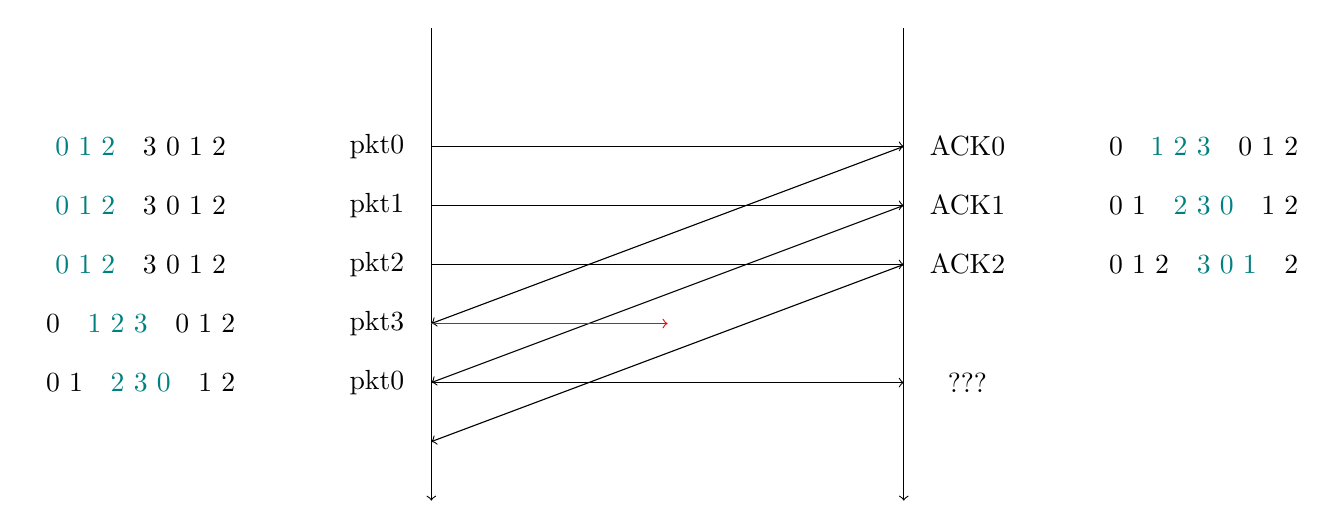
\begin{tikzpicture}[x=1.5cm, y=0.75cm]
                            \node at (-2.5, -2) {\teal{~0 1 2~}~ 3 0 1 2~};
                            \node at (-2.5, -3) {\teal{~0 1 2~}~ 3 0 1 2~};
                            \node at (-2.5, -4) {\teal{~0 1 2~}~ 3 0 1 2~};
                            \node at (-2.5, -5) {~0 ~\teal{~1 2 3~}~ 0 1 2~};
                            \node at (-2.5, -6) {~0 1 ~\teal{~2 3 0~}~ 1 2~};
                            \node at (-0.5, -2) {~pkt0~};
                            \node at (-0.5, -3) {~pkt1~};
                            \node at (-0.5, -4) {~pkt2~};
                            \node at (-0.5, -5) {~pkt3~};
                            \node at (-0.5, -6) {~pkt0~};
                            \node at (6.5, -2) {~0 ~\teal{~1 2 3~}~ 0 1 2~};
                            \node at (6.5, -3) {~0 1 ~\teal{~2 3 0~}~ 1 2~};
                            \node at (6.5, -4) {~0 1 2 ~\teal{~3 0 1~}~ 2~};
                            \node at (4.5, -2) {~ACK0~};
                            \node at (4.5, -3) {~ACK1~};
                            \node at (4.5, -4) {~ACK2~};
                            \node at (4.5, -6) {~???~};
                            \draw
                            (0, 0) edge[->] (0, -8)
                            (4, 0) edge[->] (4, -8)
                            (0, -2) edge[->] (4, -2)
                            (4, -2) edge[->] (0, -5)
                            (0, -3) edge[->] (4, -3)
                            (4, -3) edge[->] (0, -6)
                            (0, -4) edge[->] (4, -4)
                            (4, -4) edge[->] (0, -7)
                            (0, -5) edge[->, red] (2, -5)
                            (0, -6) edge[->] (4, -6);
                        \end{tikzpicture}
                    \end{center}
                    Let the window size be $w$.
                    If the receiver is waiting for segment $m$, then the receiver's window must be $[m, m + w - 1]$.
                    Assume that none of the segments $m - w, \dots, m - 1$ have been ~ACK~ by the receiver (such as the ~ACK~ being lost on its way to the sender), therefore the sender's window is still $[m - w, m - 1]$.
                    \medskip

                    None of these segments, in the sender's window, can have a sequence number that falls in the the receiver's window.
                    In order to ensure this, the sequence number space must be at least twice the window size, hence $k \geq 2w$.
                \item
                    Assume a company has two production sites located in New York and Los Angeles respectively.
                    These sites are connected through a dedicated 1 Gbps fiber connection with a one-way speed-of-light-delay of 50 ms and communicate using TCP with a congestion window of 64 KB.
                    \begin{enumerate}[(a)]
                        \itemsep0em
                        \item What is the actual throughput (using the macroscopic description of TCP)?
                            $$\frac{\frac{3}{4} \cdot W}{\text{RTT}} = \frac{\frac{3}{4} \cdot 64 \times 10^3 \times 8}{0.05 \times 2} = 3.84 \text{ Mbps}$$
                            The window varies between $\frac{W}{2}$ and $W$, hence it has a mean of $\frac{3}{4} \cdot W$ (apparently).
                        \item
                            In order to improve efficiency, two different options are available; either replace the line with a 2 Gbps fiber, or add another 1 Gbps line in parallel.
                            Ignoring installation costs, which solution would improve the throughput?
                            And the latency?
                            \medskip

                            Neither solutions would improve the latency, as that is caused by the distance between the two locations.
                            However, the throughput cannot be improved by a 2 Gbps line, since the limitation is caused by the TCP congestion window (as shown above).
                            On the other hand, with two parallel lines, the throughput can be doubled, as data can be sent in parallel.
                    \end{enumerate}
                \item Consider sending a large file from a host to another over a TCP connection that has no loss.
                    \begin{enumerate}[(a)]
                        \itemsep0em
                        \item
                            Suppose TCP uses AIMD for its congestion control without slow start.
                            Assuming that the congestion window $W$ increases by 1 MSS every time a batch of ~ACK~s is received, and assuming approximately constant round-trip times, how long does it take for $W$ to increase from 5 MSS to 12 MSS?
                            \medskip

                            1 RTT to increase to 6 MSS, 2 RTTs to increase to 7 MSS, and so on, until 7 RTTs to increase to 12 MSS.
                            Hence it requires a total of 28 RTTs.
                        \item What is the average throughput (in terms of MSS and RTT) for this connection up through time $t = 6$ RTT?
                            \medskip

                            In the first RTT, 5 MSS is sent, then 6 MSS in the second RTT, and so on, until 10 MSS is sent in the $6^\text{th}$ RTT, as such, it sends a total of $5 + 6 + 7 + 8 + 9 + 10 = 45$ MSS;
                            $$\frac{45 \text{ MSS}}{6 \text{ RTT}} = 7.5 \cdot \frac{\text{MSS}}{\text{RTT}}$$
                    \end{enumerate}
            \end{enumerate}
        \subsubsection*{Tutorial 4 - Network Security}
            \begin{enumerate}[1.]
                \itemsep0em
                \item
                    What are the differences between message confidentiality and message integrity?
                    Can you have confidentiality without integrity?
                    Can you have integrity without confidentiality?
                    Justify your answer.
                    \medskip

                    Confidentiality ensures that only the intended recipients of a message can access the contents, whereas integrity ensures that the contents of a message are valid (not tampered with) - and the recipients can detect tampering.
                    \medskip

                    It's possible to have confidentiality without integrity, as an encrypted message may be sent from $A$ to $B$.
                    However, the message may be intercepted along the way, and a new message may be sent to $B$ - the contents haven't been revealed, but the message has been tampered with, hence integrity is broken.
                    \medskip

                    On the other hand, it's possible to have integrity without confidentiality - a file may be written in plain text on a secured server, this cannot be modified by anyone who doesn't have permission to do so (hence integrity is maintained), but it is visible to everyone (and not just the intended recipient).
                \item
                    Suppose $N$ people want to communicate with each of $N - 1$ other people using symmetric key encryption.
                    All communication between any two people, $i$ and $j$ is visible to all other people in this group of $N$, and no other person in this group should be able to decode their communication.
                    \begin{enumerate}[(a)]
                        \itemsep0em
                        \item How many keys are required in the system as a whole?
                            \medskip

                            $\frac{N(N - 1)}{2}$ keys will be needed - the first person needs $N - 1$ keys to communicate with every other person, the second person needs $N - 2$ keys, since it needs to communicate with $N - 1$ other people (but a key has already been established by the first person).
                        \item
                            Now suppose that public key encryption is used.
                            How many keys are required in this case?
                            \medskip

                            Since each person has a public and private key, only $2N$ keys will be required.
                    \end{enumerate}
                \item
                    Can you decrypt a hash of a message to get the original message?
                    Explain your answer.
                    \medskip

                    No, by the definition of a hash - it is a one-way function.
                    It may however be reversed with a rainbow table, which has pre-computed values for input strings.
                \item
                    In the BitTorrent P2P file distribution protocol, the seed breaks the file into blocks, and the peers redistribute the blocks to each other.
                    Without any protection, an attacker can easily wreak havoc in a torrent by masquerading as a benevolent peer and sending bogus blocks to a small subset of peers in the torrent.
                    These unsuspecting peers then redistribute the bogus blocks to a other peers, which in turn redistribute the bogus blocks to even more peers.
                    Thus, it is critical for BitTorrent to have a mechanism that allows a peer to verify the integrity of a block, so that it doesn't redistribute bogus blocks.
                    Assume that when a peer joins a torrent, it initially gets a ~.torrent~ file from a fully trusted source.
                    Describe a simple scheme that allows peers to verify the integrity of blocks.
                    \medskip

                    Each block should have an associated hash, which is stored in the ~.torrent~ file.
                    When a peer receives a block, it should compute the hash of the received block, and compare it to the ~.torrent~ file.
                    If it matches, then the block is valid, and can be redistributed, otherwise it has been tampered with, and should be discarded.
                \item
                    Give one reason why a firewall might be configured to inspect incoming traffic.
                    Give one reason why it might be configured to inspect outgoing traffic.
                    Do you think the inspections are likely to be successful?
                    \medskip

                    Incoming traffic may be inspected by a firewall as a method of user authentication.
                    Another reason for incoming traffic to be analysed would be to detect attacks, by spotting patterns in access.
                    \medskip

                    On the other hand, outgoing traffic may be inspected to prevent data from being leaked, or to prevent a user from accessing blocked content.
                    Typically, the inspections are likely to be successful, as it can analyse the contents of the message, instead of just the headers.
                    This inspection isn't very useful however, if the contents are encryption.
            \end{enumerate}
\end{document}